% 2961w - 30p


%---------------------------------------------
%
%       THIS IS THE HIGHLIGHTED VERSION.
%       For the final version, carefully remove:
%       '\protect'
%       '\hl{' (don't forget the '}'
%
%---------------------------------------------

\documentclass[12pt,letterpaper]{article}
\usepackage{natbib}

%Packages

\usepackage{xcolor}
\usepackage{color,soul}
\usepackage{pdflscape}
\usepackage{fixltx2e}
\usepackage{textcomp}
\usepackage{fullpage}
\usepackage{float}
\usepackage{latexsym}
\usepackage{url}
\usepackage{epsfig}
\usepackage{graphicx}
\usepackage{amssymb}
\usepackage{amsmath}
\usepackage{bm}
\usepackage{array}
\usepackage[version=3]{mhchem}
\usepackage{ifthen}
\usepackage{caption}
\usepackage{hyperref}
\usepackage{amsthm}
\usepackage{amstext}
\usepackage{enumerate}
\usepackage[osf]{mathpazo}
\usepackage{dcolumn}
\usepackage{lineno}
\usepackage{dcolumn}
\usepackage{hyphenat}
\usepackage[T1]{fontenc}
\usepackage{textcomp}
\newcolumntype{d}[1]{D{.}{.}{#1}}

\pagenumbering{arabic}


%Pagination style and stuff
\linespread{2}
\raggedright
\setlength{\parindent}{0.5in}
\setcounter{secnumdepth}{0} 
\renewcommand{\section}[1]{%
\bigskip
\begin{center}
\begin{Large}
\normalfont\scshape #1
\medskip
\end{Large}
\end{center}}
\renewcommand{\subsection}[1]{%
\bigskip
\begin{center}
\begin{large}
\normalfont\itshape #1
\end{large}
\end{center}}
\renewcommand{\subsubsection}[1]{%
\vspace{2ex}
\noindent
\textit{#1.}---}
\renewcommand{\tableofcontents}{}
%\bibpunct{(}{)}{;}{a}{}{,}

%---------------------------------------------
%
%       START
%
%---------------------------------------------

\newcommand{\disp}{\texttt{dispRity} }

\begin{document}

%Running head
\begin{flushright}
Version dated: \today
\end{flushright}
\bigskip
\noindent RH: dispRity package.

\bigskip
\medskip
\begin{center}

\noindent{\Large \bf \disp: a modular \texttt{R} package for measuring disparity.} 
\bigskip

\noindent {\normalsize \sc Thomas Guillerme$^1$$^,$$^*$}\\
\noindent {\small \it 
$^1$Imperial College London, Silwood Park Campus, Department of Life Sciences, Buckhurst Road, Ascot SL5 7PY, United Kingdom.\\}
\end{center}
\medskip
\noindent{*\bf Corresponding author.} \textit{guillert@tcd.ie}\\  
\vspace{1in}

%Line numbering
\modulolinenumbers[1]
\linenumbers

%---------------------------------------------
%
%       ABSTRACT
%
%---------------------------------------------

\newpage
\begin{abstract} 

    \begin{enumerate}
        \item Biological data is multivariate in essence: many traits in organisms co-vary with each other in space and time.
        This causes biologists to either reduce these \hl{to} a manageable number of variables or, increasingly, to use multivariate toolkits.
        One such toolkit is based on creating a multidimensional space where the variables are the \hl{axes}.
        It is then possible to \hl{measure divers aspects of the distribution of some observation (e.g. species) in this space}.
        For example, if studying morphology, one can create a morphospace for two groups of species, measure \hl{the multidimensional volume occupied by each of these groups and then test whether these two volumes are significantly different or not}.

        \item There are as many definition of these multidimensional spaces, metrics and tests as there are questions that can be tackled with such methods.
        Many of these methods are implemented in specific software or R packages.
        However, the definition of the space, metric and test is often dependent on the software/package's author's point of view or specific question.
        This can unfortunately hamper researchers \hl{ability} to apply different methods that \hl{best suits} their specific questions.

        \item Here I present the \disp package, a flexible R package for running multidimensional analysis.
        This package allows users to define each step of the analysis (whether it is the space, the metric or the test) through a highly modular architecture where each definition can be passed as a function.
        It also provides a tidy interface through the \disp object, allowing \hl{users} to easily run reproducible multivariate analysis.

        \item The \disp package also comes with an extend manual regularly updated following users questions or suggestions.
        Furthermore, the package contains some simulation tools (e.g to simulate complex multidimensional space or morphological data).
        Finally it also contains a suit\hl{e} of utilities to work with \disp objects aimed at helping users to develop their own multidimensional metrics and/or tests.

    \end{enumerate}

\end{abstract}

\noindent (Keywords: disparity, ordination, multidimensionality, disparity-through-time, palaeobiology, ecology)\\

\vspace{1.5in}

\newpage 

%---------------------------------------------
%
%       INTRODUCTION
%
%---------------------------------------------

\section{Introduction}

% Multidimensionality
Biological data are complex.
To understand the ecology and evolution of species we must use multiple variables that inevitably covary with each other through time and space.
One solution to this problem is to analyse these data in a multivariate framework \citep[e.g.][]{price2015predation,diaz2016global}.
Such analyses aim to capture the complex multidimensionality of biological data, while still providing outputs that are interpretable in our physical world restricted to three dimensions.
These multivariate analyses can be used to investigate changes in morphological diversity through time \citep{Close2015}, competitive replacement scenarios \citep{Brusatte12092008}, relationships among form and function \citep{diaz2016global} and even to describe the entirety of possible shapes for a group of organisms \citep{raup1966geometric}.
The biological variables in such analyses are equally diverse, including morphological traits (discrete traits like the presence or absence of a character, e.g. \citealt{brusattedinosaur2012}; and continuous traits such as lengths, e.g. \citealt{price2015predation}), life history traits \citep[e.g.][]{diaz2016global}, or even ecosystem properties \citep[e.g.][]{DonohueDim}. 

% Variety of multidimensional spaces, metrics and tests
In all these analysis, each set of multivariate traits forms a multidimensional space.
\hl{This space is represented as a matrix where rows are regarded as samples or observations (e.g. a specimen, field sites, etc.) and columns are variables or some transformation thereof (e.g. an embedding, scaling, ordination, etc. of the variables).}
These multidimensional spaces can be defined in many ways, for example as a pairwise distance matrix \citep[][and references therein]{lloyd2016estimating}, or as outputs from a principal coordinates analysis \citep[PCO;][]{Brusatte12092008}, a principal components analysis \citep[PCA;][]{zelditch2012geometric}, or a multidimensional scaling \citep[MDS;][]{DonohueDim}, among others.
The name we give to the multidimensional space tends to vary with the kinds of traits used to construct it. 
For example, when using morphological traits the multivariate space will be a morphospace, when using ecological traits it may be referred to as an ecospace or trait space.

\hl{It is then possible to measure how the observations are distributed within this space to answer related questions (e.g. ``does group A occupies more space than group B?'').
This requires the definition of a proxy for space occupancy: the disparity metric}
\citep[or index;][]{Hopkins2017}
\hl{which can be measured in a multitude of ways.}
\hl{For example, one could use a metric based on the variance or the range of each axis of space}
\citep{Wills2001, Ciampaglio2001}
\hl{, a distance (e.g. Euclidean) measured between observations}
\citep{foote1993contributions,Foote29111996}
\hl{, a more direct approximation of the hyper volume }
\citep{cornwell2006trait,DonohueDim}
\hl{, or many more }
\citep[e.g.][]{Navarrro2003MDA}.

Finally, all these different multidimensional spaces and their associated disparity metrics can be used in an equal variety of statistical tests such as non-parametric multivariate analyses of variance \citep[e.g.][]{Brusatte12092008}, multidimensional permutation tests \citep[e.g.][]{diaz2016global} or even simply by looking at the confidence interval overlaps between disparity measurements \citep[e.g.][]{halliday2016eutherian}.
In summary, there are many different ways to perform each step of a multidimensional analysis, making analyses of complexity ever more complex.

% Problems with this variety
In theory, this multitude of ways to generate and define multidimensional spaces, measure disparity within and analyse these metrics is not an issue, in fact, it allows researchers to choose both the most appropriate method for their question or data, or even to test their question using multiple methods \citep[such as][for biogeography]{matzke2013biogeobears}.
In practice, however, this is hampered by existing software implementations.
Although many software packages exist for multidimensional analysis \citep[e.g.][]{bouxin2005ginkgo,de2007ginkgo,oksanen2007vegan,adams2013geomorph,Claddis,adams2017geometric}, package maintainers/software developers choose their preferred definition of multidimensional space and disparity metric and then enforce this on users by allowing little to no flexibility.
For example, in the excellent and widely used \texttt{geomorph} package, morphological disparity analysis uses the \texttt{morphol.disparity} function that defines the multidimensional space as the ordination of the Procrustes transform of morphometric data, the disparity metric as the Procrustes variance, and uses permutation tests to test hypotheses \citep{zelditch2012geometric,adams2013geomorph,adams2017geometric}.
%Reviewer 1 minor: Explain what the Procrustes variance is. And when is it appropriate and when is not appropriate? Be more specific.
This is ideal in some cases, but in others may not be the most appropriate analysis.
This can lead to inappropriate analyses by users confined by the existing software implementations. %Oh no!

% Here comes the solution!
The aim of the \disp package is to solve such problems by providing a completely flexible framework for studying multidimensional data.
This package is based on a highly modular architecture where each crucial decision in multidimensional analysis (which data, which metric and which test) can be provided by the user.
It implements many commonly used metrics and definitions of disparity, as well as providing a simple interface for users to implement their own disparity functions.
The package is described here for the use of discrete morphological data diversity analysis but can be generalised to any type of multidimensional data (see the package vignette for more examples).

\section{Description}
In brief, the package takes a \texttt{matrix} object (the multidimensional space), 
\hl{calculates a disparity metric from the space and analyse the resulting \texttt{dispRity} object through hypothesis testing and visualisation}
(see Manuals and Vignettes below).
Some additional functions modify the multidimensional space, for example by dividing it by groups or through time and/or bootstrapping it (see Fig. \ref{Fig:workflow} and Table \ref{Tab:main_fun}).

\begin{figure}[!htbp]
\centering
   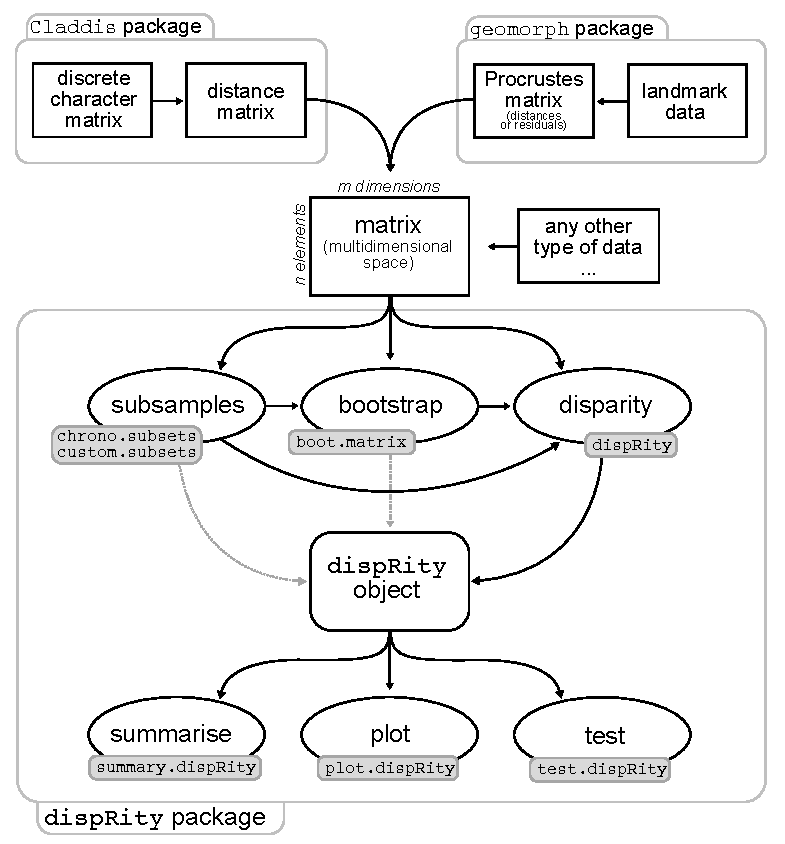
\includegraphics[width=1\textwidth]{workflowsvg.pdf} 
\caption{\disp package workflow: rectangles represent matrices; ellipses represent functions; plain black arrows indicate input/output; dashed grey arrows indicate output (though the summary, plot, and test function cannot be applied if no disparity has been calculated).}
\label{Fig:workflow}
\end{figure}

\begin{table}
    \begin{tabular}{ll}
        \hline
        Function & Description \\ 
        \hline
        \texttt{geomorph.ordination} & Imports \hl{shape} data from the \texttt{geomorph} package. \\
        \texttt{Claddis.ordination} & Imports \hl{discrete morphological} data from the \texttt{Claddis} package. \\
        \texttt{custom.subsamples} & Separates data into custom subsamples. \\
        \texttt{time.subsamples} & Separates data into time subsamples. \\
        \texttt{boot.matrix} & Bootstraps and rarefies a matrix or a \disp object. \\
        \disp & Calculates disparity from an matrix or a \disp object. \\
        \texttt{summary.dispRity} & Summarises a \disp object. \\
        \texttt{plot.dispRity} & Plots a \disp object. \\
        \texttt{test.dispRity} & Applies statistical tests to a \disp object.\\
        \texttt{dispRity.per.group} & Pipeline for \hl{disparity-within-groups} analysis. \\
        \texttt{dispRity.through.time} & Pipeline for disparity-through-time analysis. \\
        \hline
    \end{tabular}
    \caption{Main functions in the \disp package.}
    \label{Tab:main_fun}
\end{table}

\subsection{Measuring disparity}
The \disp function measures disparity of any multidimensional space (of class \texttt{matrix} or \texttt{data.frame}) where the columns correspond to the dimensions and the rows correspond to the elements present in the space.
The disparity metric (i.e. the aspect of interest of the space) is passed through the \texttt{metric} argument and is defined by the user as any function or combination of functions that can either transform the matrix into:

\begin{itemize}
    \item Another matrix (a dimension-level 3 function - e.g. a variance-covariance matrix; \texttt{stats::cor})
    \item A vector (a dimension-level 2 function - e.g. the variance of each dimension; \texttt{dispRity::variances} - see below)
    \item A single value (a dimension-level 1 function - e.g. the overall standard deviation; \texttt{stats::sd})
\end{itemize}

\begin{figure}[!htbp]
\centering
   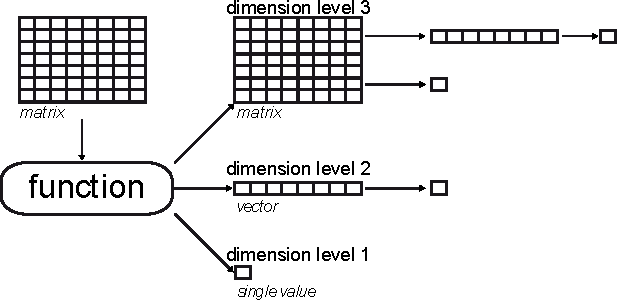
\includegraphics[width=0.8\textwidth]{../inst/gitbook/dispRity_fun.pdf} 
\caption{Illustration of the different metric dimension-levels in the \disp package. In this example, each cell correspond to a single value (e.g. a 8 $\times$ 7 matrix or a vector of eight elements).
\hl{A dimension-level 3 matrix would be a metric resulting in a matrix (e.g. the function \texttt{stats::cor} to calculate the correlation between each dimension), a dimension-level 2 metric would result in a vector (i.e. a distribution, e.g. \texttt{dispRity::variances} which calculates the variance within each dimension) and a dimension-level 1 metric would result in a single value (e.g. \texttt{stats::sd} which calculates the standard deviation of the input matrix)}}.
\label{Fig:levels}
\end{figure}

The disparity metrics can be functions from other packages, defined by the user or from the \disp package (see Table \ref{Tab:metrics} for the currently implemented metrics).
When multiple functions are passed to the \texttt{metric} argument, the functions are sorted by dimension-level and applied in decreasing order to the data.
For example, if the metric is defined as \texttt{metric = c(mean, range)}, the \texttt{range} function (dimension-level 2) is first applied to the data and the function \texttt{mean} is then applied to the result (e.g. \texttt{mean(range(data))}).
There is no limitation on the metric dimensions only that at least one dimension-level 2 or 1 function must be present in the metric definition (i.e. disparity can only be defined as distribution or a single value).
\hl{Note that this function also allows to work on only a subset of dimensions via the \texttt{dimensions} argument (e.g. if only the $n$ first dimensions must be considered).}

\begin{table}
\resizebox{\textwidth}{!}
{%
    \begin{tabular}{p{2cm}|p{5cm}|p{1cm}|p{5cm}|p{5cm}}
        name & description & dimen-sion level & definition & source \\
        \hline
        \texttt{ellipse. volume}$^1$ & The volume of the ellipsoid & 1 & $\frac{\pi^{k/2}}{\Gamma(\frac{k}{2}+1)}\displaystyle\prod_{i=1}^{k} (\lambda_{i}^{0.5})$ & \cite{DonohueDim}\\
        \texttt{convhull. surface} & The surface of the convex hull & 1 & NA & \texttt{geometry::convhulln} \\
        \texttt{convhull. volume} & The volume of the convex hull & 1 & NA & \texttt{geometry::convhulln} \\
        \texttt{diagonal} & The greatest Euclidean distance & 1 & $\sqrt{\sum_{i=1}^{k}|max(k_i) - min(k_i)|}$ & This package \\
        \texttt{mode.val} & The modal value & 1 & NA & This package\\
        \texttt{ranges} & The absolute ranges of each dimension & 2 & $|max(k_i) - min(k_i)|$ & This package \\
        \texttt{variances} & The variance of each dimension & 2 & $\sigma^{2}{k_i}$ & This package \\
        \texttt{centroids} & The distance between each element and a fixed point$^2$ of the space & 2 & $\sqrt{\sum_{i=1}^{n}{({k}_{n}-Centroid_{k})^2}}$ & This package \\
        \texttt{ancestral. distance} & The distance between an element and its ancestor & 2 & $\sqrt{\sum_{i=1}^{n}{({k}_{n}-Ancestor_{k})^2}}$ & This package \\
    \end{tabular}
}%
    \caption{\small{Where $k$ is the number of dimensions, $n$ the number of elements, $\lambda_i$ is the eigenvalue of each dimensions, $\sigma^{2}$ is their variance and $Centroid_{k}$ is their mean. $^1$ this function uses a fast estimation of the eigenvalue that only works in an ordinated space based on MDS or PCO/PCoA (\textit{not} PCA); $^2$ by default that point is the centroid of the elements.}}
    \label{Tab:metrics}
\end{table}

%TG: Add the proper sources for the convhulln package

\subsection{Splitting the multidimensional space into subsets}
Prior to calculating disparity, the multidimensional space can be subdivided into subsamples, typically to be compared to each other.
For example, one may be interested in seeing how the disparity of a specific subsample of the space compares to another (e.g. difference among groups) or, how different subsamples change sequentially (e.g. through time).
In essence, the original space corresponds to the overall space (e.g. a morphospace contains all the observed morphologies).
Conversely, subsamples correspond to parts of the space with pooled characteristics (i.e. only a subset of the total morphospace).

This splitting can be done using the \texttt{custom.subsamples} or \texttt{time.subsamples} functions.
\hl{The first argument is the matrix}
defining the multidimensional space and a list of elements to group into different subsamples.
The second also takes a matrix and arguments giving the age of the taxa (a phylogeny and/or a table containing the first and last occurence data for all/some elements - this allows species with a longer timespan to be present in multiple time subsamples for example, 
\hl{see below}
) and which subsamples to create: (1) discrete time subsamples (or time-binning) or (2) continuous time subsamples (or time-slicing).

The time-binning method groups elements by specific age range.
The time-slicing method works by using a phylogeny and looking at which taxa are present at any specific point in time.
This method thus requires the nodes to be part of the multidimensional space, a dated phylogeny (chronogram) and which model to use when slicing through branches rather than tips and nodes.
When a slice occurs not on a tip or a node, four methods are available to select either the descendent or the ancestor's node/tip as an element for this time slice:
\begin{itemize}
    \item ``acctran'' (accelerated transformation) where the data chosen along the branch is always the one of the descendant
    \item ``deltran'' (delayed transformation) where the data chosen along the branch is always the one of the ancestor
    \item ``punctuated'' where the data chosen along the branch is randomly chosen between the descendant or the ancestor
    \item ``gradual'' where the data chosen along the branch is either the descendant or the ancestor depending on branch length
\end{itemize}

\subsection{Bootstrapping and rarefying}
Disparity measurement can be influenced by sampling \citep{Butler2012}.
To take this source of bias into account, it is common practice to bootstrap the multidimensional space (to minimise the effect of outliers) or/and to rarefy the data (to minimise the effect of different sample sizes in different subsamples).
Additionally, if disparity is defined as a dimension-level 1 metric, it can be useful to measure it on bootstrapped data to obtain a distribution on which to perform statistical analyses.

Bootstrapping can be achieved by using the \texttt{boot.matrix} function which pseudo-replicates the multidimensional space following two algorithms (1) the ``full'' algorithm where the bootstrapping is entirely stochastic ($n$ elements are replaced by any $m$ elements drawn from the data) and (2) the ``single'' algorithm where only one random element is replaced for each pseudo-replicate (somewhat akin to jackknife resampling).

% In the case of disparity being a dimension-level 1 metric, it is important to note that the distribution resulting from a bootstrap will be a pseudo-replicated one and thus might not be suitable for some specific parametric statistical tests.
% Conversely, it is possible to use a dimension-level 2 metric on a bootstrapped multidimensional space to avoid this problem: the disparity metric is then measured on a pseudo-replicated multidimensional space rather than the metric itself being pseudo-replicated.

Similarly, rarefaction can be achieved through the same \texttt{boot.matrix} function.
Rarefaction can be useful when looking at the effect of reducing the number of elements on the results of an analysis or for allowing the comparisons of subsamples with the same number of elements in each.
In practice, rarefaction limits the number of elements to be drawn for each bootstrap replication: only $n-x$ elements are selected at each bootstrap replicate (where $x$ is the number of non-sampled elements).

\subsection{Interpreting results}
The functions above all generate a \disp object that can be summarised or plotted using the \texttt{S3} method functions \texttt{summary.dispRity} and \texttt{plot.dispRity} (provided disparity was calculated).
These results can then be analysed using the \texttt{test.dispRity} function for comparing subsamples or testing hypotheses.

\subsubsection{Summarising and plotting}
The \texttt{summary.dispRity} and \texttt{plot.dispRity} functions allow users to set which central tendency and which quantiles should be represented.
% as common arguments which central tendency (e.g. if central tendency is the mean and disparity was calculated as the sum of the variances for each dimensions, the central disparity tendency would be the mean of the sum of the variances) and the quantiles to represent (in the same example, if the quantile chosen is the 50th, these functions will also display 50\% of the sum of variances around the mean).
Additionally, the \texttt{plot.dispRity} function graphically represents the summarised results using different representations: (1) ``continuous'' for displaying continuous disparity curves (in the case of disparity-through-time analysis for example) and (2) ``box'', ``lines'', or ``polygons'' to display them using boxplots, confidence interval lines or polygons respectively.
Additional arguments specific to \disp objects can also be used such as \texttt{observed} to display the observed disparity (i.e. non-bootstrapped) or \texttt{rarefaction} to only plot the disparity for a certain number of elements (i.e. the rarefaction level).
The function can also take any additional graphic arguments (\texttt{main}, \texttt{xlab}, \texttt{col}, etc...) from base R.
% Note that if the disparity has been calculated on fully rarefied data (using \texttt{boot.matrix(data, rarefaction = TRUE)} prior to calculating disparity), the rarefaction curves for the whole multidimensional space (or its sub-samples) can be plotted using \texttt{rarefaction = ``plot''}.

\subsubsection{Testing hypotheses}
The \texttt{test.dispRity} function allows users to test hypotheses on the disparity data (e.g. by comparing the different subsamples to each other).
Similarly to the \disp function described above, this function can take any test defined by the user or from other R packages.
The \texttt{comparison} arguments indicates in which order (if any) the tests should be applied to the subsamples: (1) ``pairwise'' for pairwise comparisons; (2)``referential'' for comparing the first subsample to all the others; (3) ``sequential'' for comparing subsamples sequentially (e.g. first against second, second against third, etc.); (4) `all'' for comparing all the subsamples simultaneously (i.e. \texttt{disparity $\mathtt{\sim}$ subsamples} - this can be used for \texttt{lm} or \texttt{glm}) or (5) any list of pairs (or more) of subsamples to compare.

Some tests are implemented within the package such as the Bhattacharrya Coefficient \citep[\texttt{bhatt.coeff};][]{Bhattacharyya,GuillermeCooper} or a permutation test based on null hypothesised multidimensional space following \cite{diaz2016global} (\texttt{null.test}).
Additionally, this function also allows additional arguments such as \texttt{rarefaction} (as described above) or \texttt{correction} to adjust p-values when using multiple parametric tests.

\section{Examples}
Multivariate analysis can be really useful for looking
 \hl{at} 
 multiple aspects of organisms diversity together.
For example, one classic univariate trait used in ecology and evolution can be the number of species present in a ecosystem or/and through time.
This trait can be useful to test whether some ecosystems or/and time periods have more species diversity than others.
In this case one can then test some hypothesis such as: environments with
 \hl{longer altitudinal} 
 gradients contain more species.

Conversely, in the case of species diversity, one can also look at another independent multivariate trait: the diversity of morphologies \citep[or disparity;][]{ruta2013}.
Using disparity, it is then also possible to assess whether one ecosystem or/and time period display more morphological variation.
Following the previous example, if disparity is also higher with
 \hl{longer altitudinal} 
 gradients, one could argue that the species richness is caused by an increased number of morphologies adapted to more ecological niches (or something akin).

The following example is based on a classical palaeobiology morphological disparity analysis.
Note that more examples are available in the package manual (\url{https://rawgit.com/TGuillerme/dispRity/master/inst/gitbook/_book/index.html}).

\subsubsection{\disp data}
The package contains a dataset that is a subset from \cite{beckancient2014} and includes:

\begin{itemize}
    \item \texttt{BeckLee\_mat50}: an ordinated matrix for 50 mammals based on the distance between discrete morphological characters.
    \item \texttt{BeckLee\_mat99}: the same matrix \texttt{BeckLee\_mat50} but also containing the reconstruction of their 49 ancestors.
    \item \texttt{BeckLee\_tree}: a chronogram with the 50 mammal species present in \texttt{BeckLee\_mat50} and \texttt{BeckLee\_mat99}.
    \item \texttt{BeckLee\_ages}: the first and last occurrence data for 14 of the mammal species present in \texttt{BeckLee\_mat50} and \texttt{BeckLee\_mat99}.
    \item \texttt{disparity}: a pre-made \disp object based on the data above.
\end{itemize}

In this example, the multidimensional space is defined as a morphospace: the ordination of the distances among discrete morphological characters for 50 mammal species \citep[from][]{beckancient2014}.
Additionally, we can define disparity as the sum of the variances on each dimension \citep{Wills1994} that will represent an aspect of the the volume of the morphospace (i.e. a large sum of variances approximates a large morphospace and vice versa).

\subsection{Typical disparity among groups analysis}
One typical question with such analysis would be to test whether two groups of species have a different disparity.
For example, using the data described above, we can test whether the crown mammals are more diverse in term of morphology than the stem ones.
In other words, whether the approximation of the volume within the morphospace (the disparity as defined above) is different in crown or stem mammals.

\noindent These two groups can be defined as follows (where the integers are the row number of the species in the matrix):

\noindent \texttt{> mammal\_groups <- list(\textquotedbl crown\textquotedbl = c(16, 19:41, 45:50), \textquotedbl stem\textquotedbl = c(1:15, 17:18, 42:44))}

\noindent It is then possible to measure the disparity between the two groups as follows:

\noindent \texttt{> disparity <- dispRity.per.group(data = BeckLee\_mat50, group = mammal\_groups, metric = c(sum, variances))}

\noindent Note that this function is a wrapper function that is the equivalent to:

\noindent \texttt{> subsamples <- custom.subsamples(data = BeckLee\_mat50, group = mammal\_groups)}\\
\noindent \texttt{> bootstraps <- boot.matrix(subsamples)}\\
\noindent \texttt{> disparity <- dispRity(bootstraps, metric = c(sum, variances))}\\

\noindent Which allows a finer tuning of the optional arguments in each function.
The three arguments here are defined as follows: \texttt{data = BeckLee\_mat50} is our definition of the multidimensional space, \texttt{group = mammal\_groups} indicates which mammals belong to which group and \texttt{metric = c(sum, variances)} is our definition of disparity. 

This function returns a \disp object that summarises the disparity analysis:

\noindent \texttt{> disparity}\\
\noindent \texttt{ ---- dispRity object ---- }\\
\noindent \texttt{2 customised subsamples for 50 elements with 48 dimensions:}\\
          \texttt{crown, stem.}\\
\noindent \texttt{Data was bootstrapped 100 times (method:"full").}\\
\noindent \texttt{Disparity was calculated as: c(sum, variances).}\\

\bigskip
As indicated, the \disp object contains two customised subsamples (called ``crown'' and ``stem'') from a morphospace made of 50 elements for 48 dimensions.
The \disp object also displays information on the number and method of the bootstrap replicates as well as the definition of disparity.
To visualise the actual disparity values, one can use the \texttt{summary} or/and \texttt{plot} options (Table \ref{Tab:summary_group} and Fig. \ref{Fig:plot_group}):


% mammal_groups <- list("crown" = c(16, 19:41, 45:50), "stem" = c(1:15, 17:18, 42:44))
% subsamples <- custom.subsamples(data = BeckLee_mat50, group = mammal_groups)
% bootstraps <- boot.matrix(subsamples)
% disparity <- dispRity(bootstraps, metric = c(sum, variances))

\noindent \texttt{> summary(disparity)}

\begin{table}[ht]
\centering
\begin{tabular}{rlrrrrrrr}
  \hline
 & subsamples & n & obs & bs.median & 2.5\% & 25\% & 75\% & 97.5\% \\ 
  \hline
1 & crown &  30 & 2.00 & 1.93 & 1.87 & 1.92 & 1.95 & 1.98 \\ 
  2 & stem &  20 & 1.72 & 1.63 & 1.53 & 1.60 & 1.66 & 1.69 \\ 
   \hline
\end{tabular}
\caption{Summarising a \disp object (disparity per groups). $n$ is the number of elements per subsamples, $obs$ the observed disparity (not bootstrapped), $bs.median$ is the median bootstrapped disparity (here the median of the sum of ranges) and the 2.5, 25, 75 and 95\% are the confidence intervals.}
\label{Tab:summary_group}
\end{table}

\noindent \texttt{> plot(disparity)}

\begin{figure}[!htbp]
\centering
   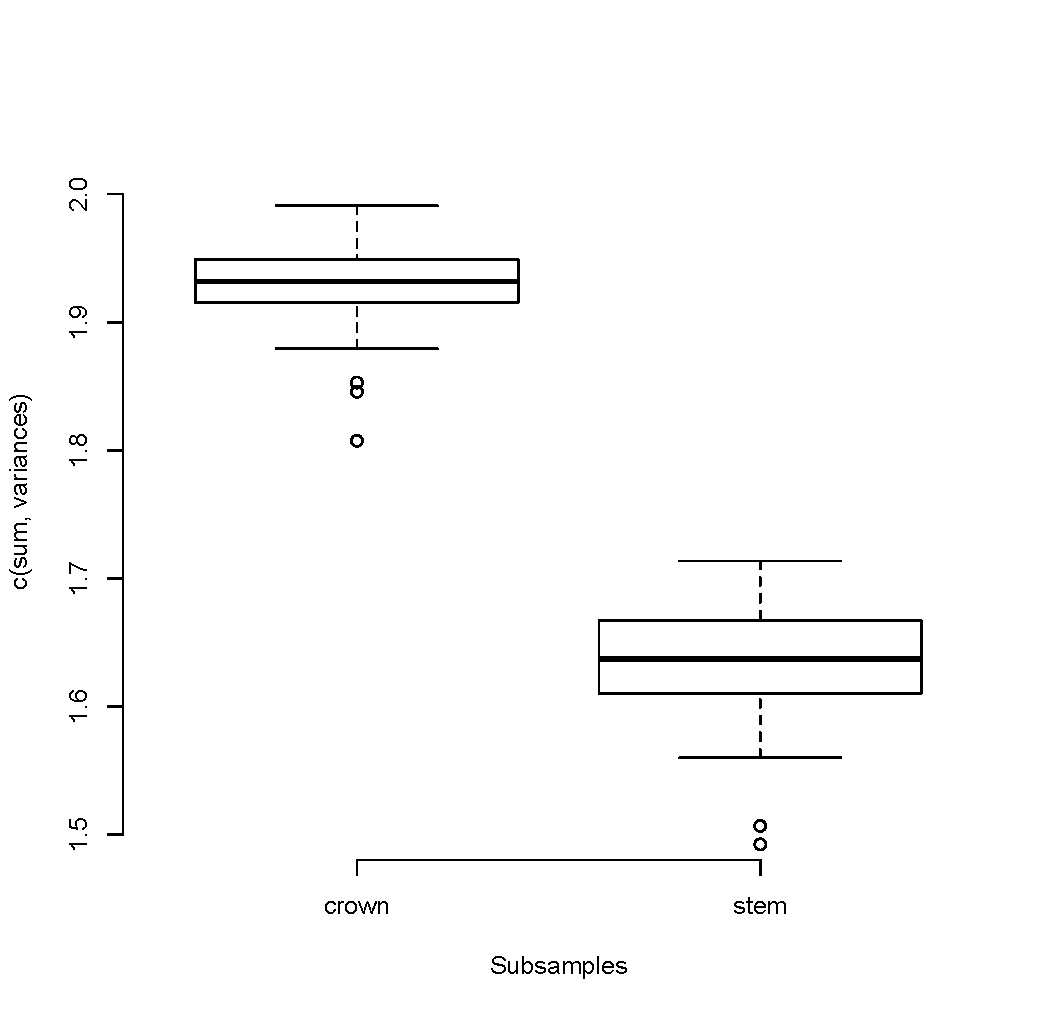
\includegraphics[width=1\textwidth]{plot_example_group.pdf} 
\caption{\disp plot of disparity differences between groups.}
\label{Fig:plot_group}
\end{figure}

As we can see from the summary table (Table \ref{Tab:summary_group}) and the plot (\ref{Fig:plot_group}), there seems to be a significant difference in morphospace volume occupied between the two groups.
It is possible to test this hypothesis by using, for example, a non-parametric Wilcoxon test (\texttt{stats::wilcox.test}):

\noindent \texttt{> test.dispRity(disparity, test = wilcox.test)}\\

\noindent \texttt{[[1]]}\\
\noindent \texttt{             statistic}\\
\noindent \texttt{crown : stem     10000}\\
\noindent \texttt{ }\\
\noindent \texttt{[[2]]}\\
\noindent \texttt{                  p.value}\\
\noindent \texttt{crown : stem 2.562144e-34}\\

\bigskip
As indicated by the p value, there is a significant difference in disparity between the groups.
Relating back to our question: yes, crown mammals display a higher diversity in morphologies than their stem counterparts (in this example and dataset!).

\subsubsection{Typical disparity-through-time analysis}
A 
\hl{subsequent} 
question to this observation could be to test whether this difference is due to an overall change in disparity through time or not.
In other words, did disparity increase through time in mammals globally or is it only between stem and crown mammals.
Using the same definition of the multidimensional space and disparity as in the previous example, we can measure, for example, changes in disparity through time between the Late Cretaceous (100.5 to 66.0 million years ago - Mya), the Paleocene (66.0 to 56.0 Mya) and the Eocene (56.0 to 33.9 Mya).

\noindent \texttt{> time\_bins <- c(100.5, 66, 56, 33.9)}

It is then possible to measure disparity-through-time using the following function:

\noindent \texttt{> disparity <- dispRity.through.time(data = BeckLee\_mat50, tree = BeckLee\_tree, time = time\_bins, metric = c(sum, variances))}

\noindent Note that this function is a wrapper function that is the equivalent to:

\noindent \texttt{> subsamples <- time.subsamples(data = BeckLee\_mat50, tree = BeckLee\_tree, time = time\_bins, method = \textquotedbl discrete\textquotedbl)}\\
\noindent \texttt{> bootstraps <- boot.matrix(subsamples)}\\
\noindent \texttt{> disparity <- dispRity(bootstraps, metric = c(sum, variances))}\\

\noindent The arguments \texttt{data = BeckLee\_mat50} and \texttt{metric = c(sum, variances)} are the same as in the example above.
However, in this type of analysis, we also need to have additional arguments: the \texttt{time = time\_bins} indicates the boundaries of the different time bins, the \texttt{tree = BeckLee\_tree} argument provides information on the age of each element and \texttt{method = 'discrete'} indicates that the data is time-binned.

Again, the resulting \disp object can be summarised and plotted (Table \ref{Tab:summary_time} and Fig. \ref{Fig:plot_time}):

\noindent \texttt{> summary(disparity)}

\begin{table}[ht]
\centering
\begin{tabular}{rlrrrrrrr}
  \hline
 & subsamples & n & obs & bs.median & 2.5\% & 25\% & 75\% & 97.5\% \\ 
  \hline
1 & 100.5 - 66 &  15 & 1.67 & 1.55 & 1.40 & 1.51 & 1.58 & 1.65 \\ 
  2 & 66 - 56 &   9 & 1.88 & 1.69 & 1.43 & 1.63 & 1.77 & 1.83 \\ 
  3 & 56 - 33.9 &  13 & 1.96 & 1.83 & 1.62 & 1.77 & 1.86 & 1.90 \\ 
   \hline
\end{tabular}
\caption{Summarising a \disp object (disparity through time). $n$ is the number of elements per subsamples, $obs$ the observed disparity (not bootstrapped), $bs.median$ is the median bootstrapped disparity (here the median of the sum of ranges) and the 2.5, 25, 75 and 95\% are the confidence intervals.}
\label{Tab:summary_time}
\end{table}

\noindent \texttt{> plot(disparity, type = \textquotedbl continuous\textquotedbl)}

\noindent Note that many plot options specific to \disp objects are available such as plotting disparity in a ``continuous'' fashion (inferring disparity between the time bins).

\begin{figure}[!htbp]
\centering
   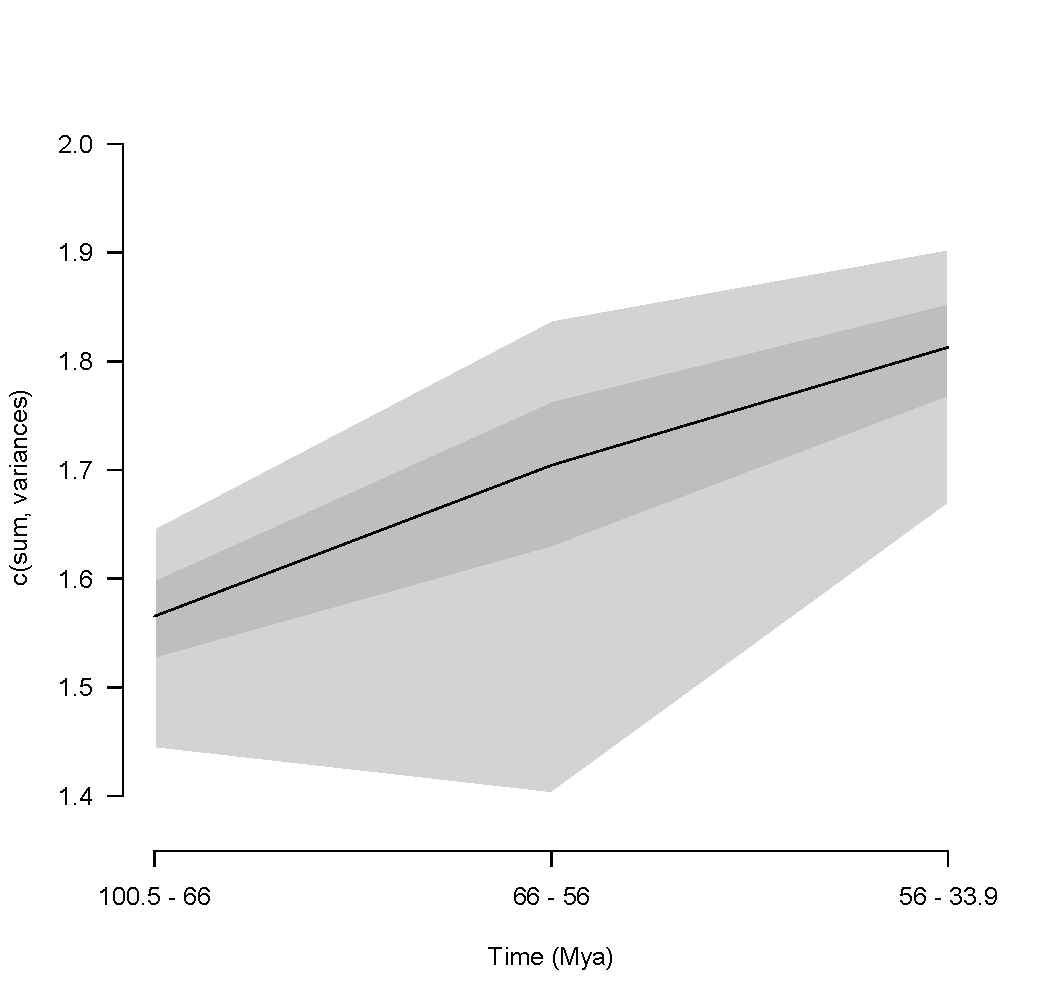
\includegraphics[width=1\textwidth]{plot_example_time.pdf} 
\caption{\disp plot of disparity-through-time. The black line represents the median disparity (median sum of variances), the dark grey and light surfaces represent respectively the 50\% and 95\% confidence intervals.}
\label{Fig:plot_time}
\end{figure}

From the plot and the summary, disparity seems to change (increase) through time from the Cretaceous to the Eocene.
Similarly to the example above, it is also possible to statistically test this hypothesis using, for example, an ANOVA (Table \ref{Tab:anova}): 

\noindent \texttt{> anova(test.dispRity(disparity, test = lm, comparisons = \textquotedbl all\textquotedbl))}

\begin{table}[ht]
\centering
\begin{tabular}{lrrrrr}
  \hline
 & Df & Sum Sq & Mean Sq & F value & Pr($>$F) \\ 
  \hline
subsamples & 2 & 3.14 & 1.57 & 177.84 & 0.0000 \\ 
  Residuals & 297 & 2.62 & 0.01 &  &  \\ 
   \hline
\end{tabular}
\caption{ANOVA performed on a \disp object.}
\label{Tab:anova}
\end{table}

To answer our specific question above: yes there is an effect of time on morphological disparity (an increase) in this dataset.

\section{Additional information}
\subsection{Manuals and vignette}
Supplementary information about the package is available on the project page (\url{https://TGuillerme/dispRity}).
Information concerning each function can be found in R in the individual function manuals and a package manual with more detailed information is available online (\url{https://rawgit.com/TGuillerme/dispRity/master/inst/gitbook/_book/index.html}).
This manual contains substantially more information and detailed examples including a tutorial for a ``classic'' disparity analysis in palaeobiology as well as an introduction to the use of this package in ecology or other disciplines. 

\subsection{Data simulations}
This package also contains functions for simulating random discrete morphological matrices (\texttt{sim.morpho}) or random multidimensional spaces (\texttt{space.maker}).
These functions are based on a similar modular architecture as that used by the \disp functions, allowing users to provide their own distribution parameters for the simulations.
For example, \texttt{stats::rnorm} can be provided as an argument for drawing normal characters rates with \texttt{sim.morpho} or normally distributed multidimensional space with \texttt{space.maker}.
The discrete morphological data simulations are based on protocols from \cite{GuillermeCooper}, \cite{OReilly20160081} and \cite{puttick2017uncertain}. 
The multidimensional space simulations are based on the methods from \cite{diaz2016global}.
Both functionalities are described in more details in the package manual.

% \subsection{Further directions} TG: maybe this section is useless
% Further functionalities and improvement on current functionalities will be implemented in future versions.
% In fact, optimised architecture and a C implementations are being currently developed for faster calculations and lower memory footprints for most computational heavy functions (e.g. \disp or \texttt{time.subsamples}).
% New functionalities currently being developed will include time sequential linear models (for accurately measuring directionality in disparity changes between time slices) or mode of disparity evolution testing (allowing to fit different models such as Brownian Motion or Ornstein-Uhlenbeck to disparity curves).

\section{Conclusion}
The \disp package is based on a highly modular architecture allowing researchers to simply define both their multidimensional space and their disparity metric to efficiently analyse multivariate data.
The \disp object allows users to easily pipeline disparity analysis from the data input (the matrix) to publication standard results (tables, plots, hypothesis testing).

% \section{Data availability and reproducibility}
% All the code and the data for using the package and its vignette with examples are available in the R package help files or on GitHub \url{github.com/TGuillerme/dispRity}.

\section{Acknowledgments}
Many thanks to Natalie Cooper for encouraging the development of this package and helping with the writing of this paper and the package manuals.
Thanks to Martin Brazeau and Andrew Jackson for specific implementation ideas 
\hl{and to Michael Collyer, Gavin Simpson and two other anonymous reviewers for constructive comments on the earlier version of this manuscript}. %TG: add Graeme Lloyd, Dave Bapst and Emma Sherratt
I acknowledge support from European Research Council under the European Union's Seventh Framework Programme (FP/2007 – 2013)/ERC Grant Agreement number 311092 awarded to Martin D. Brazeau 
\hl{and from the Discovery Project Grant DP170103227 awarded to Vera Weisbecker}.


\section{Funding}
This work was funded by the European Research Council under the European Union's Seventh Framework Programme (FP/2007–2013)/ERC Grant Agreement number 311092 
\hl{and the Discovery Project Grant number DP170103227}.

\bibliographystyle{sysbio}
\bibliography{References}

\end{document}
